%%=============================================================================
%% Methodologie
%%=============================================================================

\chapter{\IfLanguageName{dutch}{Methodologie}{Methodology}}
\label{ch:methodologie}

%% TODO: Hoe ben je te werk gegaan? Verdeel je onderzoek in grote fasen, en
%% licht in elke fase toe welke stappen je gevolgd hebt. Verantwoord waarom je
%% op deze manier te werk gegaan bent. Je moet kunnen aantonen dat je de best
%% mogelijke manier toegepast hebt om een antwoord te vinden op de
%% onderzoeksvraag.



Na de stand van zaken die gebaseerd is op de literatuurstudie volgt de volgorde van stappen die ondernomen zijn om deze proef te voltooien. 

\section{z/OS Health Checker standaard setup}
\label{sec:z/OS Health Checker Standaard setup}

De eerste onderzoeksvraag was of er mogelijkheid was tot een standaardopstelling binnen de z/OS Health Checker omgeving van HCL Technologies. Maar eerst moet er een analyse plaatsvinden op de huidige opstelling van Health Checker. Om deze te optimaliseren

\subsection{Analyse van huidige z/OS Health Checker Setup}
\label{subsec:Analyse van huidige z/OS Health Checker Setup}
De opstelling die in deze proef geanalyseerd werd bevind zich binnen een parallel sysplex. En deze parallel sysplex werken we met 4 LPARS: VT1, VT2, VT3 en VT4. Elke LPAR heeft verschillende checks. Maar na de 4 LPARS te overlopen was het duidelijk dat de meeste checks op VT1 draaien. Daarom is de analyse gefocust op VT1.

De analyse is gemaakt met de check data uit SDSF deze kan je bereiken door bij het ISPF hoofdmenu volgende optie te geven 's;ck'. Dit is S voor SDSF met als volgende optie CK voor Health Checker deze ziet er zo uit.

\begin{figure}[h]
	\centering
	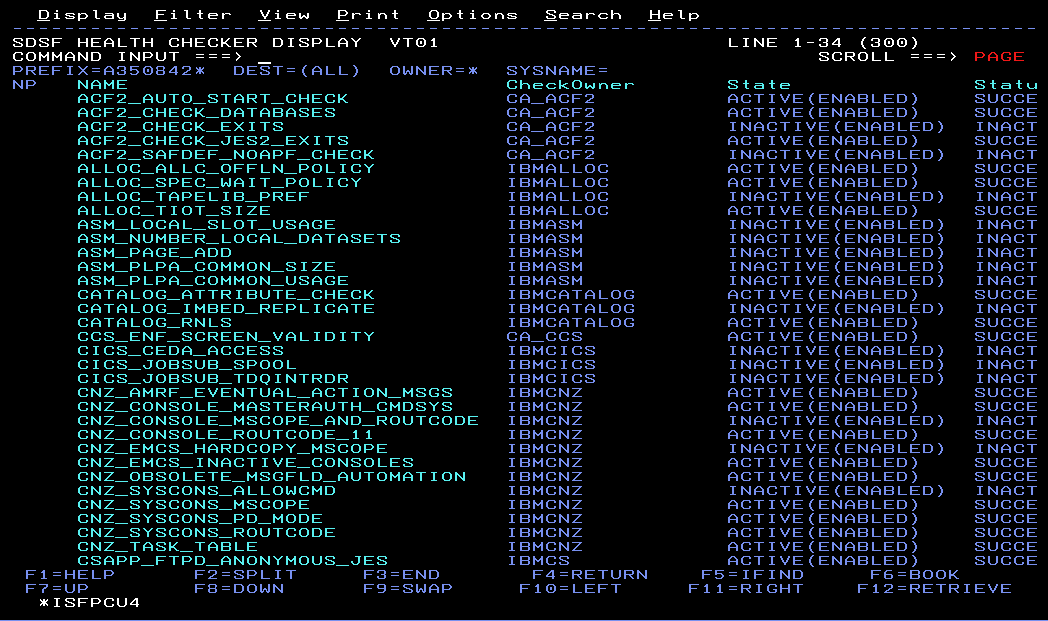
\includegraphics[width=0.7\linewidth]{img/SDSFCK}
	\caption[Health Checker Scherm binnen SDSF]{Dit is het Health Checker paneel binnen SDSF hier kunnen we de output van de laatste keren dat een check is uitgevoerd}
	\label{fig:sdsfck}
\end{figure}


Na het overlopen van alle checks op VT1 zijn deze samengevat zoals volgende tabel. Met de naam van de check. De status, deze beschrijft of de check aanstaat of niet. De outcome, deze beschrijft of de check succesvol was of niet. En de reason, dit is de reden waarvoor de check draait.

\begin{tabular}{|p{5cm}|p{3.5cm}|p{1.5cm}|p{5cm}|}
	\hline
	\textbf{Name} & \textbf{Status} & \textbf{Outcome} & \textbf{Reason} \\
	\hline
	XCF\_CDS\_MAXSYSTEM & ACTIVE(ENABLED) & SUCCES & CDS MAXSYSTEM value across all CDS types should be at least equal to the value 
	in the primary sysplex CDS.  \\
	\hline
\end{tabular}

Maar sommige checks hebben GLOBAL als outcome. Dit betekent dat de check niet op de huidige LPAR draait maar op een andere. Global checks draaien voor de gehele sysplex maar moeten maar op 1 LPAR geactiveerd staan.
